\documentclass[11pt]{article}
\usepackage{graphicx}
\usepackage{courier}

\title{Detecting ``Fake News" on Facebook}
\author{Hannah Eyre\\ Zane Zakraisek}
\usepackage[margin=1.0in]{geometry}


\begin{document}
\maketitle

The term ``Fake News" gained popularity during the United States' 2016 Presidential Election to describe a rapidly spreading phenomena of news articles deliberately spreading false information and hoaxes, often through attention grabbing headlines or headlines that resemble legitimate sources \cite{guardian}. It became particularly notorious on social media sites and Facebook in particular, where the top 20 articles from hoax sites and hyperpartisan blogs garnered more user interaction between August 1st and election day on November 8th than the top 20 articles from a variety of established news sources such as {\it The New York Times}, {\it Washington Post}, {\it Business Insider}, and Fox News \cite{buzzfeed}.

FactCheck.org, part of the Annberg Public Policy Center at the University of Pennsylvania, breaks down how an individual can identify fake news into eight parts \cite{factcheck}:
\begin{enumerate}
\item Consider whether the source is credible.
\item Read beyond the headline.
\item Check whether the author is credible or real.
\item Check whether the article is recent.
\item Check whether it is a joke or satire.
\item Consider your own biases and how they affect your judgment.
\item Check supporting sources (if any) and make sure they abide by the same rules.
\item Ask experts or fact-checking sites.
\end{enumerate}

Rapidly spreading fake news articles have a range of consequences, one instance culminating in a gunman attacking a Washington, DC pizza parlor over allegations of child pornography and child sex abuse ring centered around John Podesta, Hillary Clinton's 2016 campaign manager, in a conspiracy called ``Pizzagate" \cite{pizzagate}. Various politicians and government agencies in the United States and internationally have voiced opinions on what qualifies as fake news and what do do about it, but no consensus has been reached. Facebook was initially reluctant to admit there was any problem with fake news on news feeds, however Facebook's CEO Mark Zuckerberg has since released a statement describing how they plan to deal with fake news in the future, including renaming the phenomenon ``false news" \cite{zuckerberg}.

As an increasingly global and hotly contested issue, we would like to to explore what responsibility Facebook has in regards to these eight points. We will discuss whether they have a responsibility to develop tools to detect fake news based off these guidelines and, if these tools exist, whether they should be used to remove content from the site.

\paragraph{Why we're choosing to minimize negative utility}

\section{Credible sources: Zane}
\section{Reading Beyond the Headline}

When posting an external link to Facebook, information is drawn from the content inside \texttt{meta} elements of the page source by Facebook's web crawler and placed into a preview on the post itself. If an element labeled according to the Open Graph protocol, the crawler will place it in the link preview on the site \cite{fbwebmaster}. With this system in place, every linked website will appear the same on a users news feed. Any site can determine how its posts show up when linked on Facebook, regardless of the quality of the content or site itself. \\

\begin{figure}[h]
	\begin{minipage}{0.48\textwidth}
		\centering
		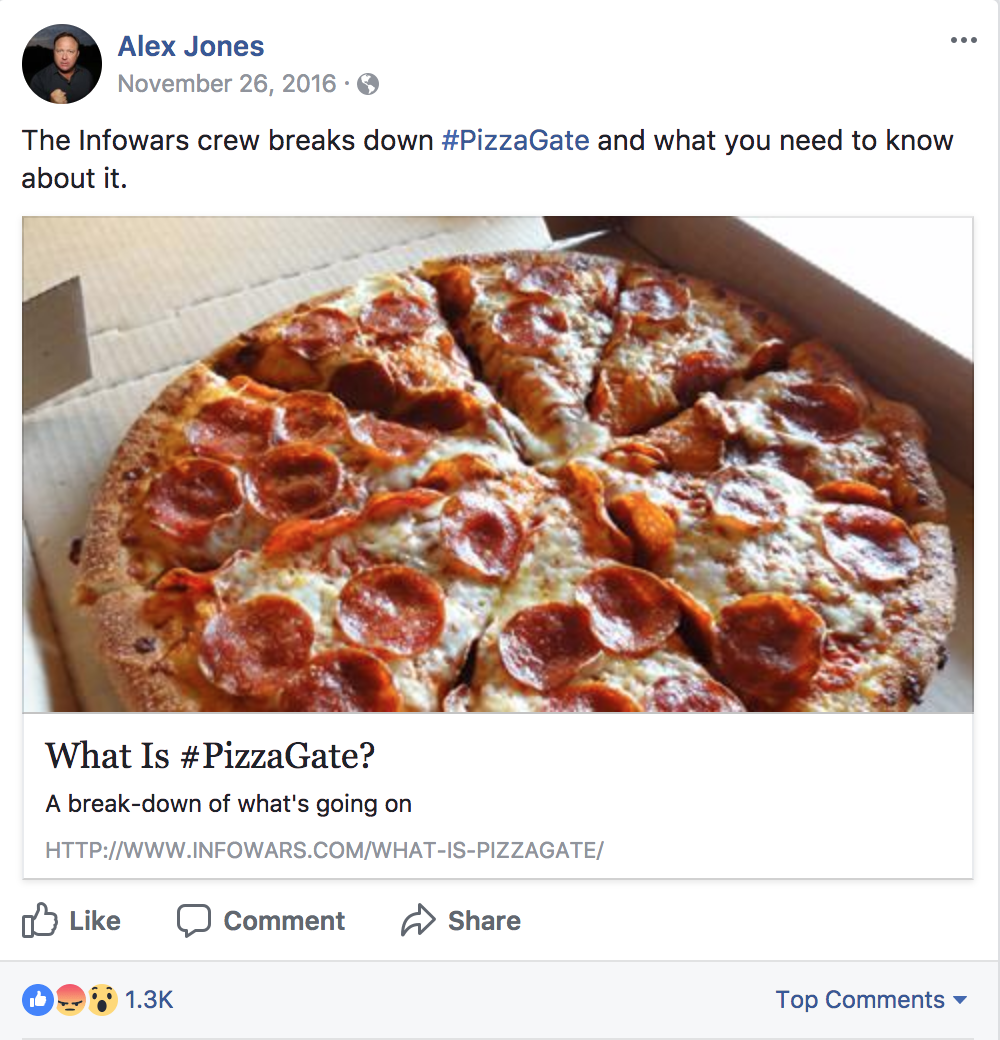
\includegraphics[scale=.3]{pizzagate_alex_jones_fb}
	\end{minipage}
	\begin{minipage}{0.48\textwidth}
		\centering
		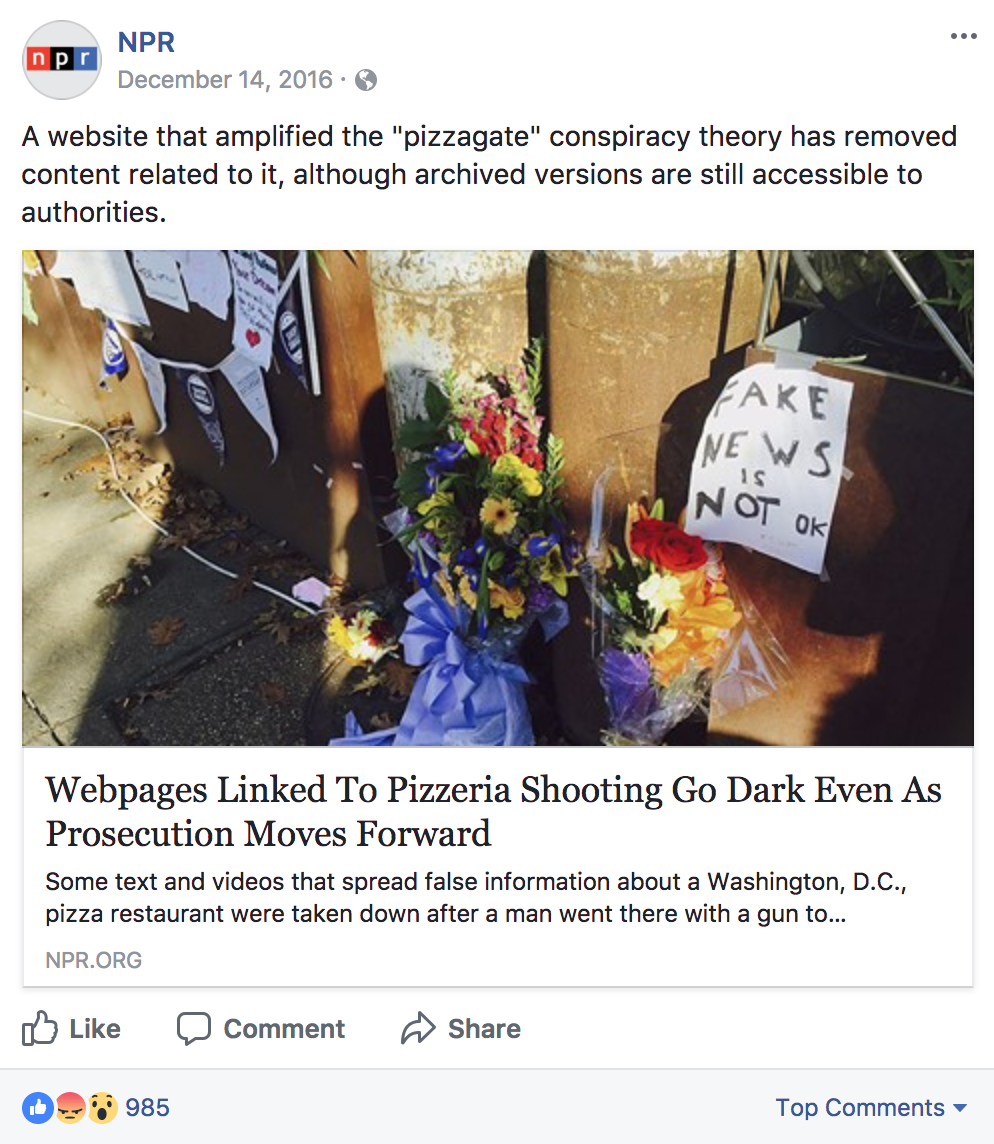
\includegraphics[scale=.3]{pizzagate_npr_fb}
	\end{minipage}
	\caption{A comparison of posts by Alex Jones, creator of {\it Infowars}, \cite{alex_jones_pizzagate_post} and {\it NPR} \cite{npr_pizzagate_post} about Pizzagate.}
\end{figure}

This uniform formatting treats {\it NPR} and {\it Infowars} or any other site that uses the \texttt{meta} elements according to Facebook's specifications as equals. It places less emphasis on the source of the article than on the headline and picture. The examples above are posted from official accounts, allowing users to easily see where the article comes from. However, the same articles posted by friends or unofficial pages make the source more difficult to determine.

In addition, because the information taken by the Facebook crawler is entirely determined by the web developer, the headline, picture, and description can be completely misleading.

\section{Author Credibility: Zane}
\section{Age of the Article: Hannah}
Considering the age of the article is an important aspect of identifying fake news. Both very recent articles and older articles can be subject to scrutiny.

Manipulating trending topics with new, uninformed articles

quoting old sources with no date

\section{Article Genre: Hannah}

the onion, dedicated satire site, https://www.theonion.com/no-way-to-prevent-this-says-only-nation-where-this-r-1819580358

new yorker, sometime satire, 

"just a joke" defense for harassment, 

\section{Interpretation Bias: Hannah}

facebook demographics, http://journals.sagepub.com/doi/abs/10.1177/2053168017720008

trending topic staff fired, https://www.theguardian.com/technology/2016/aug/29/facebook-fires-trending-topics-team-algorithm

\section{Article Sources: Zane}
\section{Cross Reference: Zane}

\paragraph{Final utility based on points above}

\newpage
\bibliographystyle{apalike}
\bibliography{proposal_bibliography.bib}


\end{document}
